\section{Modulation}
	On va voire comment greffer l'information sur un signal.
	
	La \textbf{modulation} permet de transposer un signal (signal modulant) autour d'une autré fréquence (fréquence porteuse). Le signal modulé ressemble a une sinusoide et la variation contient l'information du signal modulant:
	\begin{equation}
		v_x(t) = A_c \cos(w_ct + \varphi_c)
	\end{equation}
	Il y a 3 type de modulation:
	\begin{itemize}
		\item modulation d'amplitude (joue sur $A_c$)
		\item modulation de fréquence (joue sur $w$)
		\item modulation de phase (joue sur $\varphi_c$)
	\end{itemize}
	
	dans cette section nous allons voire la modulation analogique
	
	\subsection{Modulation en bande de base}
		Bon j'ai m'enti il y en a 4.
		La transmition est dite en bande de base si elle ne subit aucune transposition de fréquence par modulation. Les fréquences initials du signal émis sont donc préservé.
	\subsection{Modulation d'amplitude (AM)}
		
		\begin{figure}[htp]
			\centering
			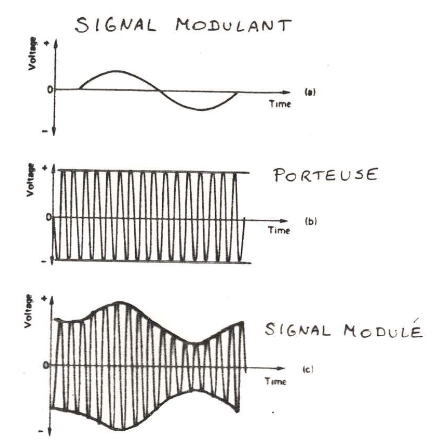
\includegraphics[width=0.4\textwidth]{img/modulationAM.png}
		\end{figure}
		
		Avec une porteuse et un signal modulant, on crée le signal modulé en appliquant les changements d'amplitude du signal modulant. Avec $s(t)$ le signal et l'on sait que $\varphi_c = 0$ on a :
		\begin{equation} \label{eq1}
			\begin{split}
		v_x(t) &= A_c \cos(w_ct + \varphi_c) \\
		v_{AM}(t) &= A_c \cos(w_ct) + ms(t) A_c \cos(w_c t) \\
		& = A_c[1+ms(t)]\cos(w_c t)
			\end{split}
		\end{equation}
		
		L'amplitude est multiplié par $(1+ms(t))$. Si $m$ (indice de modulation) est trop grand on a une \textbf{surmodulation} et donc une perte de l'information
		\begin{figure}[htp]
			\centering
			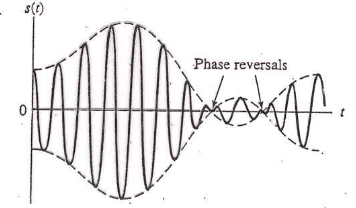
\includegraphics[width=0.4\textwidth]{img/surmodulation.png}
		\end{figure}
		
		\subsubsection{Modulation autour d'un porteuse}
			Rappel de Fourier:
			\begin{equation} \label{eq1}
			\begin{split}
				f(t) &\Leftrightarrow F(\omega)\\
				f(t-t_0) & \Leftrightarrow F(\omega) \exp(-jwt_0)\\
				f(t) \exp(jt\omega_0) &\Leftrightarrow F(\omega - \omega_0)\\
				f(t) \exp(-jt\omega_0) &\Leftrightarrow F(\omega + \omega_0)\\
				f(t) \cos(\omega_0 t) &\Leftrightarrow \cfrac{F(\omega + \omega_0) + F(\omega - \omega_0)}{2}
			\end{split}
		\end{equation}
		
		\begin{figure}[htp]
			\centering
			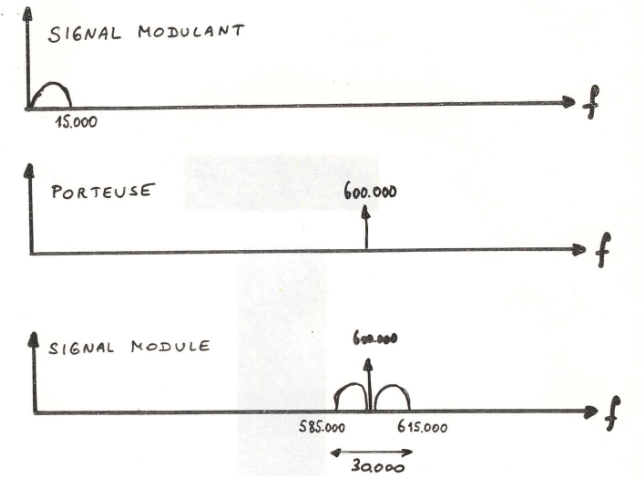
\includegraphics[width=0.4\textwidth]{img/modulationAM1.png}
			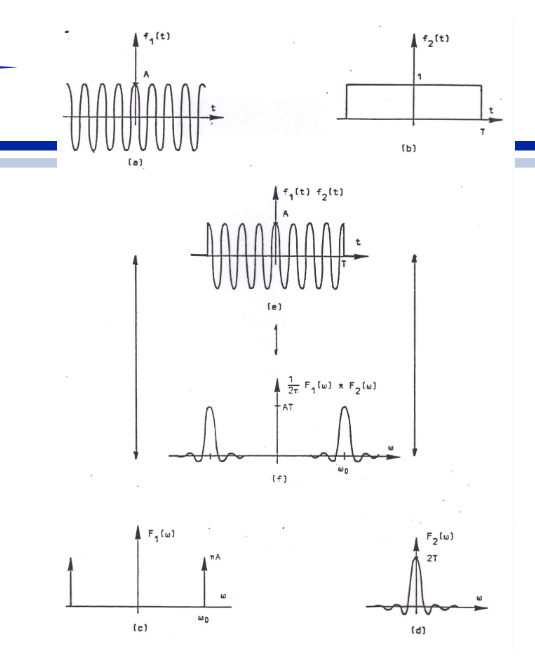
\includegraphics[width=0.4\textwidth]{img/modulationAM2.png}

		\end{figure}
			
		Multiplier le signal par la porteuse $\cos(\omega_0 t)$ en terme de Fourier, consiste de décaler le spectre des fréquences de $\omega_0$ dans les 2 sens autour de la porteuse. Il y aura donc des fréquences "\textit{négative}"
			
		\begin{figure}[htp]
			\centering
			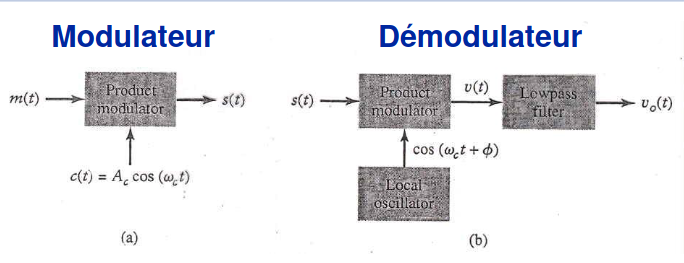
\includegraphics[width=0.6\textwidth]{img/modulationAM3.png}
		\end{figure}
		
		\textbf{Modulation :} le signal modulant $m(t)$ multiplié par une cosinusoïde résulte par le signal modulé $s(t)$
	
		\textbf{Démodulation :} le signal modulé $s(t)$ multopilié par la meme cosinusoïde que pour la modulation resulte en $v(t)$ et permet de retrouver le signal d'origine autour de la fréquence 0 sur la lequel on vient d'appliquer un filtre passe-bas pour conserver que le signal qui nous interesse.
			
			
		Le signal sortant du démodulateur ressemble a :
		
		\begin{equation} \label{eq1}
			\begin{split}
				p(t) &= A_c s(t) cos (\omega_c t + \varphi_c).\cos(\omega_c t + \varphi_c)\\
				&= A_c s(t) cos^2 (\omega_c t + \varphi_c).\cos(\omega_c t + \varphi_c)\\
				&= A_c s(t) \cfrac{A + cos(2\omega_c t + 2\varphi_c)}{2}
			\end{split}
		\end{equation}
		
		On va filtrer en passe-bas pour retrouver $s(t)$
		
		\subsubsection{Filtrage}
			Permet de filtrer un signal résultant d'un modulateur pour garder les composant interessant du contenu fréquentiel
			
			\begin{figure}[htp]
			\centering
			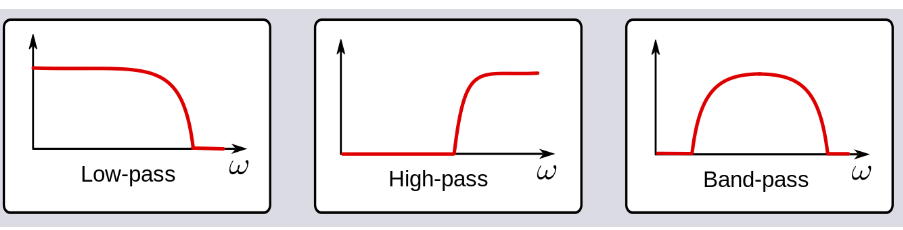
\includegraphics[width=0.6\textwidth]{img/filtrage.png}
			\end{figure}
			
			la fréquence de coupure $(freq_{coup})$
			
			\begin{itemize}
				\item \textbf{Filtre passe-bas (low-pass)} : Garde les composantes du contenu fréquentiel \textbf{en dessous} de la $freq_{coup}$ et retire celle \textbf{au dessus}
				\item \textbf{Filtre passe-haut (High-pass)} : Garde les composant du contenu fréquentiel \textbf{au dessus} et retirer celle \textbf{en dessous}
				\item \textbf{Filtre passe-bande (Band-pass)} : Garde les composantes du contenu fréquentiel \textbf{entre} la $freq_{coup\_1}$ et la $freq_{coup\_2}$ (ou $freq_{coup\_1} < freq_{coup\_2}$) et retire le reste.
			\end{itemize}
		
		\subsubsection{Bandes latérales}
			Comme dit précédemment, de fréquence "négatives" sont envoyé il est donc inutile d'envoyé 2 fois la meme info. Envoyé 2 bande latéral est suffisant que on reconstruit apres. Il y a 2 moyen pour savoir quelle bande envoyé.
			\begin{itemize}
				\item USB (upper side band) envoi les deux aux extrémité
				\item LSB (Lower side band) envoi les 2 au centre
			\end{itemize}
			
						
			\begin{figure}[htp]
			\centering
			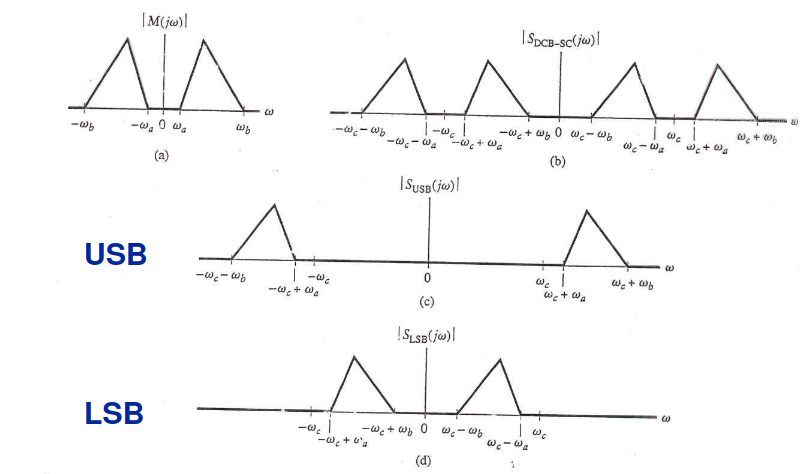
\includegraphics[width=0.6\textwidth]{img/BandeLateralUnique.png}
		\end{figure}
		
	\subsection{A CONTINUER}